\documentclass[thesis.tex]{subfiles}
\begin{document}
\chapter{Background and Related Work}
\label{cha:cha2}

\section{Introduction}

In this chapter, we will discuss related works of various subfields of English text simplification, as well as text generation more generally. This chapter is broken down into six main sections. First, Section \ref{sec:lexical_review} discusses lexical simplification, the most well-researched sub-task of text simplification involving identifying complex words within a text, and replacing them with simpler words that preserve the meaning of the original sentence. This section also discusses various commonly-used resources used for lexical and phrasal substitution and simplification. This section is most relevant for the work involved in Chapter \ref{chap:lexical}, though the idea of understanding textual complexity is something that is discussed throughout this thesis.

Next, Section \ref{sec:data_review} focuses on the main text simplification corpora leveraged by these sentence-level statistical systems, and later neural-based systems as well, to learn common simplification operations. In particular, we consider Parallel Wikipedia, which aligns sentences from Simple Wikipedia articles with their corresponding Wikipedia articles \citep{zhu2010monolingual}; and also Newsela, a dataset of news articles re-written at five complexity levels by professional editors \citep{xu2015problems}. These corpora, especially Newsela, are critical in many paraphrasing, generation, and retrieval experiments in Chapters \ref{chap:lexical}, \ref{chap:sentence}, and \ref{chap:retrieval}, respectively.

Section \ref{sec:statistical_review} focuses on phrase-based and statistical text simplification systems. These systems still attempt to address lexical and phrasal substitution, but also attempt to address other common sub-tasks such as deletion, reordering, and sentence splitting. These models often create statistically-driven components for each subtask, before combining them together into a pipeline to holistically simplify a sentence. This work is generally considered the state-of-the-art approach to text simplification prior to the rise of neural-based methods. Note that this is a trend common to machine translation, dialogue systems, and many other generation tasks.

After this, Section \ref{sec:seq2seq} focuses on the rise of neural-based approaches, both within text simplification and across natural language processing. We first provide a high-level description of the structure of a basic Sequence-to-Sequence (Seq2Seq) model \citep{sutskever2014sequence}, which typically involves an initial model that \textit{encodes} an input into some latent representation, and a second model that takes this representation and uses it to \textit{decode} an output one token at a time. Next, we discuss several applications of Seq2Seq approaches to sentence simplification, which we use as a basis of comparison for our own sentence simplification models in Chapter \ref{chap:sentence}. Finally, we discuss several standard approaches for effectively decoding an output from a Seq2Seq model. These include greedy search, which involves simply taking the most likely token from the probability distribution at each time step; and beam search, which involves keeping track of the $k$ most likely partial sequences throughout the decoding process. This section serves as a basis for the various diverse decoding approaches discussed some in Chapter \ref{chap:sentence}, but especially in Chapter \ref{chap:decoding_strategies}.

Section \ref{sec:eval_background} considers various methods for evaluating sentence simplification systems. We first discuss the three main dimensions upon which systems are evaluated: fluency, adequacy, and relatively complexity. We consider several metrics that attempt to approximate human judgments on these three dimensions when comparing to a single reference sentence or multiple reference sentences. After this, we also consider quality estimation metrics, which attempt to estimate the quality of a generated simple sentence \textit{without a reference}. These metrics are used significantly in Chapter \ref{chap:sentence}, both as ways to evaluate the quality of our own sentence simplification models, as well as the basis of comparison for the creation of our own metric.


Lastly, Section \ref{sec:lm_review} briefly discusses large-scale pre-trained language models that have revolutionized nearly every aspect of natural language process in recent years. In particular, we focus on BERT, a contextual word embedding model trained on two very general language understanding tasks with a vast amount of data \citep{devlin2019bert}. We discuss the importance of these language models on their own, but that the most noteworthy property of these models is that they can be fine-tuned on a small amount of task-specific data to significantly outperform models trained from scratch. We refer to BERT-based models throughout all Chapters: in Chapter \ref{chap:lexical} we perform a posthumous comparison of our models to RoBERTa-based approaches; in Chapter \ref{chap:sentence} we fine-tuned BERT to estimate the quality of sentence simplification systems; in Chapter \ref{chap:decoding_strategies} we use BERT to cluster similar sentences together; and in Chapter \ref{chap:retrieval} we leverage BERT-based models both for identifying critical concepts, for predicting document-level complexity, and ultimately for retrieving related documents at various complexity levels.

\section{Lexical Simplification} \label{sec:lexical_review} 

\subsection{Disambiguation-based and Direct Methods}

Lexical simplification is a sub task of text simplification, which involves replacing complex words in a text with simpler substitutes that preserve their meaning. Lexical simplification can involve identifying complex words in context \citep{shardlow2013cw}, substitute generation \citep{biran2011putting}, and finally choosing the appropriate substitute for each complex word.

To identify the words to be simplified, \cite{shardlow2013comparison} proposes to use a Support Vector Machine (SVM) that exploits several lexical features, such as token length, token frequency, number of characters, and number of syllables. Our best approach in Chapter \ref{chap:lexical} also integrates a SVM classifier for identifying complex words, but complements this set of features with context-related and embedding-based features that have not been exploited in previous work.

In lexical simplification, existing methods differ as to whether they include a word sense disambiguation (WSD) step for substitute selection, and in the ranking method used. Ranking is often performed based on word frequency in a large corpus, since it has been shown that frequent words increase a text's readability \citep{devlin1998use,kauchak2013improving}. Models that include a semantic processing step for substitute selection aim to ensure that the selected substitutes express the correct meaning of words in specific contexts. WSD is often carried out by selecting the correct synset (i.e. set of synonyms describing a sense) for a target word in WordNet; the synonyms in the synset are then used as substitutes. \cite{konvens2012wordnet} use WordNet's tree structure to reduce the size of the vocabulary in a document; we discuss WordNet and other paraphrase corpora in detail in the next section. \cite{biran2011putting} perform disambiguation in an unsupervised manner. They learn simplification rules from comparable corpora and apply them to new sentences using vector-based context similarity measures to select words that are the most likely candidates for substitution in a given context. This process does not involve an explicit WSD step, and simplification is addressed as a context-aware lexical substitution task. The SemEval 2012 English Lexical Simplification task \citep{specia2012semeval} also addresses simplification as lexical substitution \citep{mccarthy2007semeval}, allowing systems to use external sense inventories or to directly perform in-context substitution.

\subsection{Lexical Semantic Resources}

One of the earliest and best-known lexico-semantic resources is WordNet, a manually curated lexical network which encodes semantic relationships between words \citep{miller1995wordnet}. WordNet contains 155,327 words grouped into 175,979 synsets, i.e. synonym sets, along with relationships between these synsets. Relationships between two synsets $S_1$ and $S_2$ include hypernymy, which occurs when the words in $S_1$ are subtypes of those in $S_2$; meronymy, which occurs when the words in $S_1$ denote parts of those in $S_2$; and antonymy, where the words in $S_1$ have opposite meaning from those in $S_2$. In addition, some words can appear in multiple distinct synsets, indicating that they have multiple meanings. For example, the word \textit{bug} is related to nouns such as \textit{insect} and \textit{beetle}, but also separately to nouns such as \textit{error} and \textit{mistake} \citep{cocos2016clustering}.

%Beyond manually curated resources, there have also been several corpora created 
Semantic resources have also been created using automatic methods. One such resource is the Paraphrase Database (PPDB), which contains more than 220 million English paraphrase pairs \citep{ganitkevitch2013ppdb,pavlick2015ppdb}. PPDB was created using a bilingual pivoting technique, which assumes that two English phrases that translate to the same foreign phrase have the same meaning \citep{bannard2005paraphrasing}. This pivoting technique was applied to a parallel corpus containing more than 106 million sentence pairs and over 2 billion English words, spanning 22 pivot languages. Word-level alignments inside the parallel sentences were done automatically, and thus do contain some noise; this results in paraphrase pairs of varying quality. In addition, PPDB paraphrases are not always synonyms, but are often categorized by other types of relationships, as in WordNet.
%While PPDB is useful on its own, the usage of automatic word alignments between the parallel sentences resulted in paraphrase pairs of varying quality. In addition, restricting PPDB to a single definition of synonymy is often too general; as discussed with WordNet, ofter other relations between paraphrase are more appropriate. 
To address these issues and promote good paraphrase pairs, the PPDB 2.0 score was introduced which reflects the strength of paraphrase relations \citep{pavlick2015ppdb}. This work also classified the relation of each paraphrase pair ($P_1$, $P_2$) as one of six entailment relations: 

\begin{itemize}
\item \textbf{Equivalence}, where $P_1$ and $P_2$ are true synonyms (e.g.,\textit{distant} vs. \textit{remote})
\item \textbf{Forward Entailment}, where $P_1$ is a specific type of $P_2$ (e.g., \textit{mosquito} vs.  \textit{bug})
\item \textbf{Reverse Entailment}, where $P_2$ is a specific type of $P_1$ (e.g., \textit{bug} vs.  \textit{mosquito})
\item \textbf{Exclusion}, where $P_1$ has the opposite meaning of $P_2$ (e.g., \textit{nobody} vs.  \textit{someone})
\item \textbf{Independent}, where $P_1$ and $P_2$ have no relation (e.g., \textit{car} vs. \textit{family})
\item \textbf{Other Related}, where $P_1$ and $P_2$ have some relation other than entailment (e.g., \textit{swim} vs. \textit{water})
\end{itemize}

In order to leverage a paraphrase resource for the task of text simplification, it is critical to know given a paraphrase pair ($P_1$, $P_2$), which phrase is simpler than the other. The Simple Paraphrase Database (SimplePPDB) was created for this purpose, which is a set of 4.5 million simplification rules extracted from PPDB \citep{pavlick2016simple}. These rules come with both the predicted strength of the paraphrase relation (PPDB 2.0 score) and a simplification confidence score. This takes into account the strength of the paraphrase relation, and how well the ride side of the rule simplifies the word on the left. For example, \textit{perish} $\rightarrow$ \textit{die} has a confidence score of 0.909, while \textit{perish} $\rightarrow$ \textit{murder} has a confidence score of 0.108. This simplification score was created by sampling 1,000 PPDB phrases, and extracting up to 10 of their paraphrases found in the resource. For each pair ($P_1$, $P_2$), crowdsourced annotations were collected which determine how well $P_2$ preserves the meaning of $P_1$, and which paraphrase is simpler than the other (or if there is no difference in complexity between the two). \cite{pavlick2016simple} train a multi-class logistic regression model on this data to predict if applying a paraphrase rule will result in a simpler or more complex output, or in an output that does not make sense. We show how we can effectively rank SimplePPDB paraphrases for an in-context lexical simplification task in Chapter \ref{chap:lexical}.

\section{Sentence Simplification Corpora} \label{sec:data_review}

One of the main problems in simplification work is collecting a reasonable amount of quality data. Early work sfocused on specific aspects of simplification, allowing systems to leverage more general corpora. The lexical simplification work of \cite{carroll1999simplifying} utilized lexico-semantic resources such as WordNet \citep{miller1992wordnet}, while work focusing on deletion \citep{filippova2008dependency} leveraged sentence compression corpora built from the British National Corpus and the American News Text Corpus. However, with the rise of statistical- and neural-based methods, which need to be trained on parallel sentences, collecting sentences containing a variety of simplification operations has become increasingly important.

\subsection{Simple Wikipedia} \label{pwkp}

In order to build an effective statistical-based system that takes into account all aspects of text simplification, \cite{zhu2010monolingual} created a corpus of parallel sentences by leveraging Wikipedia and Simple English Wikipedia, which is tailored for younger children and adult English language learners. To do this, the authors first aligned regular and Simple English Wikipedia documents by tracking the language link found in Wikipedia dumps. After segmenting the articles into sentences, \cite{zhu2010monolingual} aligned similar sentences in the aligned articles using sentence-level Term Frequency-Inverse Document Frequency (TF-IDF) \citep{nelken2006towards}. TF-IDF is a standard scoring scheme which indicates the importance of a particular word to a document within a corpus \citep{Salton1988term}. In order to compute sentence-level TF-IDF, \cite{nelken2006towards} consider each sentence as a document. They then can define the weight $w$ for a term $t$ in a sentence $s$ as follows:

\begin{equation}
    w_s(t) = TF_s(t) * \frac{N}{DF(t)}
\end{equation}

In this formula, $TF_s(t)$ represents whether or not the token $t$ is found in sentence $s$, $N$ is the total number of sentences in the corpus, and $DF$ represents the number of sentences in which $t$ is found.

The PWKP corpus has been widely used in simplification research, since it allows for the training of advanced statistical simplification systems \citep{woodsend2011learning,coster2011learning,wubben2012sentence}. However, in their descriptive statistics of the dataset, \cite{zhu2010monolingual} show that the aligned Simple English Wikipedia sentences are only slightly shorter than their corresponding Wikipedia sentences (20.87 vs. 25.01 tokens per sentence). \cite{siddharthan2014survey} further points out it is necessary to perform a more exhaustive examination of the quality of Simple English Wikipedia. The main reason is that, contrary to machine translation evaluation, which typically relies on native speakers to judge quality, it is generally difficult to find a ``native Simple English speaker" because most adult English speakers are relatively advanced. 

Taking this analysis further, \cite{xu2015problems} perform an in-depth analysis of Simple English Wikipedia and PWKP. The authors extract 200 random sentence pairs from PWKP, and find that 50\% of the pairs were either not correctly aligned (17\%) or not good examples of actual simplifications (33\%). Additionally, only 12\% of the sentence pairs feature both deletion and paraphrasing, two key operations in simplification. \cite{xu2015problems} argue that this is likely due to the fact that Simple English Wikipedia was created by volunteers, and these articles are also rarely complete rewrites of the original Wikipedia articles, often leaving much of the information out.

\begin{table}
\begin{center}
\begin{tabular}{|c|c|c|c|c|c|} \hline
Statistic & \textbf{L4} & \textbf{L3} & \textbf{L2} & \textbf{L1} & \textbf{L0} \\ \hline
\# words/doc & 1,152.01 & 996.59 & 931.78 & 799.48 & 676.20 \\
\# words/sent & 23.23 & 19.44 & 16.60 & 14.11 & 11.91 \\ \hline
\end{tabular}
\end{center}
\caption{\label{tab:newsela} Descriptive statistics depicting the difference in complexity levels in the Newsela corpus \citep{xu2015problems}. Here, \textbf{L3} is the least simplified version of the original document, while \textbf{L0} is the most simplified version.}
\end{table}

\subsection{The Newsela Corpus} \label{sec:newsela}

To reduce the field's reliance on Simple Wikipedia, \cite{xu2015problems} proposed a new corpus based on articles collected by Newsela, an education company that focuses on creating K-12 reading materials. This corpus (hereafter called Newsela V1) initially consisted of 1,130 news articles on a variety of topics, which were rewritten at four complexity levels by Newsela editors. In what follows, we describe the original document  as Level 4 (L4), and the simplified documents as Level 3 (L3) to Level 0 (L0), depending on their complexity level. Table \ref{tab:newsela} shows descriptive statistics about the complexity of documents and sentences at the five Newsela levels. We can see that L0 documents indeed have on average significantly shorter sentences, a significant improvement over PWKP.

To extract parallel sentences, \cite{xu2015problems} first align sentences from an article with complexity $c$ with the most similar sentence in the same article with complexity $c - 1$. Unlike in PWKP, sentential similarity is calculated using the proportion of overlapping lemmatized words between two sentences $s_1$ and $s_2$:

\begin{equation}
sim(s_1, s_2) = \frac{\lvert lemmas(s_1) \cap lemmas(s_2) \rvert}{\lvert lemmas(s_1) \cup lemmas(s_2) \rvert}
\end{equation}

In order to analyze the quality of the Newsela corpus, \cite{xu2015problems} manually annotate 50 sentences from each level. This experiment finds that in L2, 34\% of sentences are not simpler, while in L0, only 6\% of the sentences are considered not simpler, and 68\% had undergone both deletion and paraphrase operations. In total, this version of the Newsela corpus includes 141,582 sentence pairs.

Although the Newsela corpus was an improvement over previous datasets, the initial alignment algorithm used struggled to effectively align longer sentences, as these sentences were likely to have been changed significantly or split into multiple sentences in the simplified articles. Recently, \cite{jiang2020neural} introduced a two-step process to better align sentences from parallel corpora. This work starts with an initial paragraph alignment step. Given two paragraphs in aligned documents $p_1 \in D_{i, L(j)}$ and $p_2 \in D_{i, L(j^{\prime})}$, paragraph-level semantic similarity score ($simP$) is computed by taking an average of the maximum sentence-level similarities for each sentence $s_1 \in p_1$ and $s_2 \in p_2$). A pair of paragraphs ($p_1$, $p_2$) is considered aligned if they are both similar \textit{and} found in similar positions in their respective documents; additionally, paragraphs are aligned if two continuous paragraphs $(p_2, p_3) \in D_{i, L(j^{\prime})}$ are both relatively similar to $p_1$. 

Next, \cite{jiang2020neural} train a neural conditional random field (CRF) model to identify similar sentences within the aligned paragraphs. This model is able to leverage both sentence-level similarities as well as an alignment label transition, which accounts for the fact that if a complex sentence $c_i$ is aligned with a simple sentence $s_j$, it's likely that $c_{i-1}$ is aligned with $s_{j-1}$, and $c_{i+1}$ is aligned with $s_{j+1}$. In this work, semantic similarity is computed by fine-tuning BERT \citep{devlin2019bert} on manually labeled data. Compared with the first version, these changes result in a significant increase in sentence pairs that contain both sentence splitting and additional rewrite operations, while also increasing the number of aligned sentences to 666,645. Note that this is partially due to the second version of the Newsela corpus (Newsela V2) being larger and containing 1,882 aligned articles, but the improvements introduced in this work further increase both the quality and quantity of parallel sentences.

\section{Phrase-based and Statistical Text Simplification} \label{sec:statistical_review}

Most recent work has attempted to solve the problem of text simplification holistically, formulating the task as a monolingual translation problem. Here, the input is a complex English sentence and the output is a sentence in simplified English. Training on a large corpus of aligned sentences allows models to perform transformation operations needed for simplification simultaneously. In this section, we discuss various statistical simplification systems, which have served as building blocks for later neural-based simplification models. We discuss in detail a seminal work on combining simplification sub-tasks into a holistic system \citep{zhu2010monolingual}; a hybrid phrase-based model that has been proposed in order to better incorporate deletion and sentence splitting \citep{narayan2014hybrid}; and finally a statistical machine translation approach augmented with lexical substitutions \citep{xu2016optimizing}.

While these methods have attempted to address the problem of sentence simplification holistically, in general these models are still broken down into several sub-models. This is not always a bad idea, particularly when phenomena related to simplification are not seen much in the training data, as is often the case for sentence splitting. However, under the assumption that the data is sufficient, a single model that jointly learns to perform all aspects of simplification simultaneously would likely generate more coherent and simpler output.

\subsection{Tree-based Simplification Model}

The first work that focused on integrating simplification subtasks into a holistic sentence-level simplification system is the Tree-based simplification model (TSM) \citep{zhu2010monolingual}. This work integrates sentence splitting, deletion, reordering, and substitution operations into a single cohesive model. This work was also the first to effectively leverage Simple Wikipedia in order to collect parallel sentences.
%This dataset, known as the Parallel Wikipedia Corpus (PWKP), is discussed in more detail in Section \ref{pwkp}.

The first step in TSM is to perform sentence splitting, if needed. To do this, \cite{zhu2010monolingual} decide whether or not to split a sentence on a boundary word, such as ``which" in Figure \ref{fig:split_example}, by using the relative length of the original sentence compared to the simplified version. Subsequently, the model determines whether to drop the boundary word by considering the word itself and the corresponding constituent within the parse tree; in Figure \ref{fig:split_example}, this corresponds to ``which" and ``WHNP", respectively.

\begin{figure}
    \begin{subfigure}[c]{\textwidth}
    \centering
    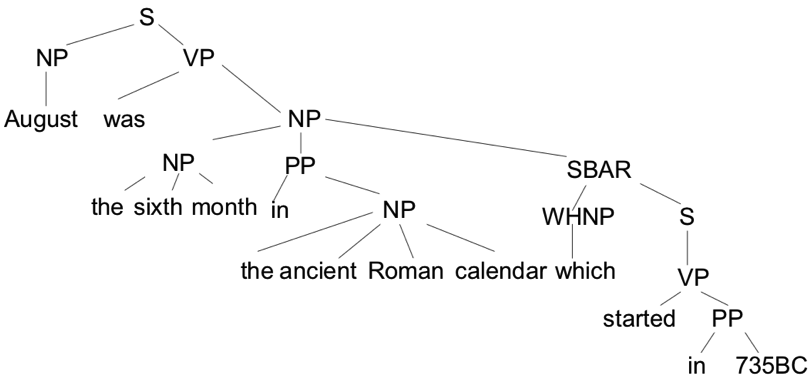
\includegraphics[width=.6\textwidth]{pictures/sentence-split1.png}
    \end{subfigure}
    \newline\newline\newline
    \begin{subfigure}[c]{\textwidth}
    \centering
    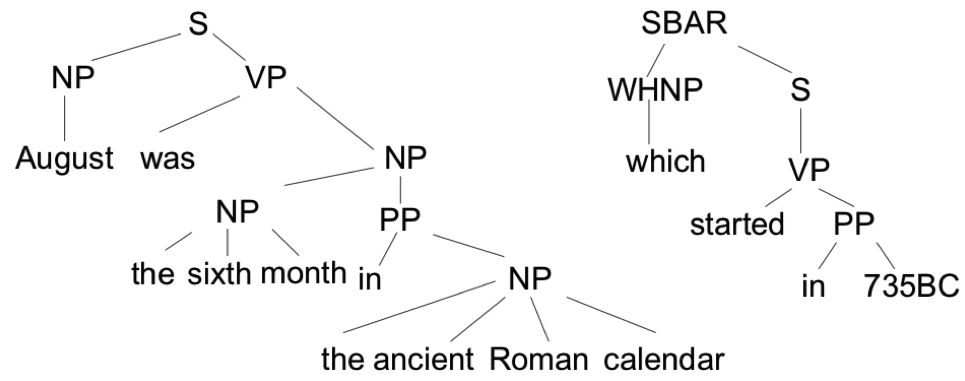
\includegraphics[width=.6\textwidth]{pictures/sentence-split2.png}
    \end{subfigure}
    \caption{A potential split based on the parse tree of the sentence, ``August was the sixth month in the ancient Roman calendar which started in 735BC.". Example recreated from \cite{zhu2010monolingual}.}
    \label{fig:split_example}
\end{figure}

Similarly, for deletion, \cite{zhu2010monolingual} utilize a word's direct parent node along with the constituent pattern of its children. In the example in Figure \ref{fig:split_example}, the phrase ``the sixth month" represents the constituent rule ``NP $\rightarrow$ DT JJ NN". The model then probabilistically determines which parts of the rule should be kept, and which can be deleted.

Finally, for substitution, \cite{zhu2010monolingual} use of a substitution table that tracks the probabilities $P(s|w)$, where $w$ is a word and $s$ is any candidate substitute for $w$. We can easily extend this to phrasal substitution by instead tracking the probabilities $P(s|n)$, where $n$ is a non-terminal node in the constituency parse. The decision to make a phrasal or lexical substitution is determined by the node $n$ having a higher probability than the most likely substitutions for all children of $n$. To calculate the probabilities in the substitution tables, these are initialized to a uniform distribution, and then updated by running an Expectation Maximization (EM) algorithm on the parallel sentences from PWKP.

Subsequent work built on the phrase-based machine translation framework by incorporating additional deletion (PBMT) \citep{coster2011learning} and post-hoc reranking (PBMT-R) \citep{wubben2012sentence} mechanisms. In addition, \cite{woodsend2011learning} presented a phrase-based model based on quasi-synchronous grammar to capture structural mismatches and complex rewrite operations.

\subsection{Adding Deep Semantics to Phrase-based Machine Translation}

While phrase-based systems such as TSM \citep{zhu2010monolingual} perform reasonably well when making simplifications at the lexical and phrasal level, they tend to perform poorly when deleting tokens and splitting sentences, two key aspects of simplification. To circumvent this problem, \cite{narayan2014hybrid} incorporate better pre-processing steps for deletion and sentence splitting, before utilizing a probabilistic phrase-based system. Regarding sentence splitting, the authors argue that a purely syntactic approach \citep{zhu2010monolingual} is often inadequate. This is because in cases where the split sentences share a phrase, relying on syntax alone often fails to correctly generate this phrase in both sentences. Instead, the authors recommend using a formal semantic representation of the sentence which is derived from Discourse Representation Theory (DRT). In particular, the Hybrid model takes as input a Discourse Representation Structure (DRS). A simple example sentence and its corresponding DRS is shown below:

\begin{itemize}
    \item \textbf{Sentence}: The man walks the dog.
    \item \textbf{DRS}: [x,y: man(x), dog(y), walks(x, y)]
\end{itemize}

With this representation, it is possible to clearly identify phrases that are shared across different parts of the sentence, and which are critical components, e.g. agents or patients.

Similarly, the authors leverages the DRS to determine what parts of the sentence should be deleted. The model can determine which phrases are crucial components, and which are optional content that can potentially be removed. In contrast, work that only considers the input sentence or the syntactic structure does not discriminate between phrases, and thus can delete important parts of the sentence.

The last component is to further simplify by making lexical and phrasal substitutions, and reordering the sentence. \cite{narayan2014hybrid} train a standard phrase-based machine translation system on PWKP. In addition, to ensure the output is relatively fluent, the authors train a general language model on Simple Wikipedia, and integrate this into their phrase-based simplification system. Altogether, the Hybrid model can be defined as follows:

\begin{equation}
    Hybrid(c) = \underset{s}{\text{argmax}}\text{ }P(DRS_c | s^{\prime}) P(s^{\prime}|s) P(s)
\end{equation}

Here, $c$ represents the original complex sentence, $DRS_c$ is the semantic representation of $c$, $s^{\prime}$ represents the intermediate sentence(s) after performing splitting and deletion, and $s$ is a candidate simplified sentence. Their results show that their hybrid method greatly outperforms previous phrase-based simplification systems in terms of simplicity, while remaining competitive on fluency and adequacy.

\subsection{Integrating Lexical Simplification into Statistical Machine Translation}

In contrast to previous phrase-based work which utilizes several components to model different aspects of simplification, \cite{xu2016optimizing} instead start from a standard statistical machine translation approach and integrate several simplification-specific aspects, focusing mainly on substitution. In addition, for substitution this work leverages the Paraphrase database (PPDB), a collection of more than 100 million English paraphrase pairs \citep{ganitkevitch2013ppdb}. While PPDB rules are not simplification-specific, the sheer size allows for much greater coverage compared to previous simplification datasets, and non-simplifying rules can subsequently be filtered out.

To properly leverage PPDB rules for simplification, \cite{xu2016optimizing} train a linear model $l_{\textbf{w}}(c, s)$, where $c$ is the original complex sentence, $s$ is the candidate simplified sentence, and $\textbf{w}$ are the weights learned by the model. As features, the authors first consider all features available in PPDB for each paraphrase pair $(p_1, p_2)$; these include the conditional paraphrase probability $P(p_2|p_1)$, the distributional similarity between the paraphrases' contexts, part-of-speech information, $n$-gram based features for words seen in the left and right of a phrase, among others. Beyond paraphrase-specific features, \cite{xu2016optimizing} also calculate paraphrase length in characters, their length in words, the maximum number of syllables, and the fraction of common English words included in the paraphrases. These features are computed for both $p_1$ and $p_2$.

In order to learn $\textbf{w}$, \cite{xu2016optimizing} use a pairwise ranking optimization algorithm, which differentiates a good simplification $s_g$ from a bad simplification $s_b$ using some automatic metric $m$. In other words, the pair $(s_1, s_2)$ is labeled as 1 if $m(c, s_1) > m(c, s_2)$, and as 0 otherwise, for some metric $m$. This work tries three metrics as $m$: BLEU, a standard $n$-gram-based metric to measure quality in machine translation \citep{papineni2002bleu}; FKBLEU, a novel metric which combines BLEU with the difference in Flesch-Kincaid Grade Level between the original sentence and the candidate \citep{kincaid1975derivation}; and SARI, a second novel metric which tracks how many $n$-grams are correctly kept, added, and deleted by the candidate. These metrics are discussed in detail in Section \ref{sec:eval_background}.

Using both automatic metrics as well as human judgments of fluency, adequacy, and number of good simplifications made (simplicity+), \cite{xu2016optimizing} find that optimizing on BLEU results in candidates that are identical to the original sentence; this is one of many experiments that demonstrates the fact that BLEU is generally not a good metric for optimizing simplification systems \citep{sulem2018bleu}. The combination of PPDB and SARI seems to perform best overall, making more simplifications while preserving fluency and adequacy better than the previous state-of-the-art system of \cite{wubben2012sentence}. However, the number of actual simplifications is still quite low compared to the reference sentences (0.65 vs 1.35).

\section{Neural Machine Translation and Applications to Simplification} \label{sec:neural_review}

Sequence-to-Sequence (Seq2Seq) models, which learn mappings from one sequence to another using a neural network, have had enormous success in not just text simplification, but also a variety of natural language processing applications, notably including machine translation \citep{sutskever2014sequence,luong2015effective,vaswani2017attention}, text summarization \citep{nallapati2016abstractive}, and dialog systems \citep{vinyals2015neural}. In this section, we first present an overview of the Seq2Seq framework, followed by a discussion of recent applications of Seq2Seq models to text simplification. We also include a description of common decoding strategies.

\subsection{Sequence-to-Sequence Models} \label{sec:seq2seq}

Seq2Seq models generally include an encoder and a decoder model. The encoder transforms some input $\textbf{x}$ into a fixed-size latent representation, $z \in \mathbb{R}^V$, while the decoder transforms this representation to output a conditional probability for each word in the target sequence, $\textbf{y}$, given the input sequence and tokens generated so far. Here, $V$ is the cardinality of the enumerated vocabulary $\mathcal{V}$. Generally, the encoder and decoder are both Recurrent Neural Networks (RNNs) \citep{sutskever2014sequence}, though more recent works have sometimes replaced these with attention-based Transformer networks \citep{vaswani2017attention}. The encoder and decoder are then jointly trained in order to maximize the conditional probability of the target sentence given the source sentence, i.e. $P(\textbf{y}|\textbf{x})$.

At every step \textit{t} of the input sequence, the encoder generates the hidden state as follows: 
\begin{equation}
	h_t = f(x_t, h_{t-1})
\end{equation}
where $x_t$ is the current token in the sentence and $h_{t-1}$ is the hidden state at the previous time step. Here, the function $f(.)$ is generally a Long Short-Term Memory (LSTM) network. The final hidden state of the encoder is then taken as the context vector $c$ to be passed to the decoder. 

At each time step $t$, the decoder generates the next token $y_t$ and its hidden state $d_t$ as follows:
\begin{equation*}
	d_t = f(d_{t-1}, y_{t-1}, c)
\end{equation*}
\begin{equation*}
    \label{eqn:seq2seq-decode}
	P(y_t|y_{1:t-1}, c) = g(d_t, y_{t-1}, c)
\end{equation*}
Here, the function $g(.)$ is a softmax layer to convert scores into a valid probability distribution.

During the decoding process, most strategies attempt to find the most likely overall sequence, i.e. choose a $\mathbf{\hat{y}}$ such that:
\begin{align*}
    \mathbf{\hat{y}} = \arg\max_{\mathbf{y}}{ P(\mathbf{y} | \mathbf{x})} = \arg\max_{\mathbf{y}}{\prod_{t=1}^{N} {P(y_t \mid y_{1:t}, \mathbf{x})}}
\end{align*}
However, unlike Markovian processes, no sub-exponential algorithm exists to find the best decoded sequence, and thus we instead use approximation algorithms. The simplest approach to decoding a likely sequence is to greedily select the most likely word at each timestep:
\begin{equation*}
    \hat{y}_t = \arg\max_{y_t}{ P(y_t | y_{1:t-1}, \mathbf{x})}
\end{equation*}

There are several key limitations in this original architecture. Since the last step of the encoder is the only thing that is passed to the decoder, it is expected to contain information from the entire sentence; this problem, known as bottlenecking, becomes increasingly problematic with longer sentences. In addition, recurrent neural networks (RNNs) that were generally used as the encoder and decoder models are generally somewhat slow to train; since each RNN step takes the output from the previous step, only one step can be computed at a time.

To address the bottlenecking problem, the concept of \textit{attention} was introduced, which allows the decoder to focus on the relevant parts of the source sentence \citep{bahdanau2014neural,luong2015effective}. With this approach, the context vector at time step $t$, $c_t$, is no longer static; instead, it now depends on the entire $sequence$ of hidden states.

\begin{equation*}
	c_t = \sum_{t=1}^{T_{\textbf{x}}} \alpha_{it}h_t
\end{equation*}

In this formula, $T_{\textbf{x}}$ represents the number of time steps in the input \textbf{x}, and $\alpha_{it}$ represents the weight of each hidden state. The decoder now receives all encoder hidden states, each of which represents the addition of a single token from the source sentence. Each step in the decoder learns a score for each encoder state, where important states are given higher scores. Finally, we take the softmax of these scores, and multiply them by the hidden states to get an overall context vector. Incorporating attention into Seq2Seq models was shown to greatly improve performance on machine translation and other generation tasks.

To speed up training, \cite{vaswani2017attention} proposed removing the RNN component of the model altogether and to rely solely on attention; this is known as the \textit{transformer} architecture. The model still consists of separate encoder and decoder components. In the original architecture, the encoder is six encoders stacked on top of each other; the decoder is set up in the same way. Each encoder contains two layers: a self-attention layer, followed by a feed-forward neural network. For each word $w$, the self-attention layer looks at the rest of the input to better encode $w$. Since the attention mechanisms has no knowledge of the position of each word in the input, before being passed into the encoder, the embeddings corresponding to the input text are modified using positional encodings. The decoding side is similarly structured, with the output from the previous decoder layer being used as input to the subsequent layer. After the decoders, there is a final linear layer, followed by a softmax layer to produce a final probability distribution over the vocabulary. Following the standard Seq2Seq framework, after each word is predicted, the output sequence so far is passed through the decoder as additional context.\footnote{This description of transformers is partially based on the blog post http://jalammar.github.io/illustrated-transformer/.} The transformer architecture is much faster to train and also delivers better results when compared to previous state-of-the-art RNN-based Seq2Seq models.

\subsection{Applications of Seq2Seq models to Text Simplification}

After the success of Seq2Seq models in machine translation and other text generation tasks, it was natural for this architecture to be applied to text simplification as well, as this has often been viewed as a monolingual machine translation task from complex to simple English. \cite{nisioi2017exploring} proposed the first major application of Seq2Seq models to text simplification, applying the standard encoder-decoder approach with attention, and using beam search as their decoding strategy. This work shows that a vanilla Seq2Seq model directly applied to text simplification is able to generate output that is more grammatical and better at preserving the meaning of the original sentence compared to previous statistical and phrase-based models.

However, although a higher proportion of the changes proposed by Seq2Seq models are high quality, they still make significantly fewer changes compared to previous approaches \citep{nisioi2017exploring}. This illustrates one of the key challenges in applying standard Seq2Seq models to simplification. If we consider sentence pairs in the Newsela dataset, 73\% of tokens are copied from the original to the simplified version in Newsela, making the copy operation by far the most common operation \citep{zhang2017sentence}. Because standard Seq2Seq models are extremely good at picking up on patterns present in the data, they naturally learn to copy very well, resulting in output that is often either identical to the original sentence, or only with a few small changes. Due to this issue, most subsequent work focuses on how to encourage the model to make more simplification operations that do not involve copying from the original.

To counteract this tendency of the models, \cite{zhang2017sentence} integrate reinforcement learning into the Seq2Seq framework. This rewards the model for producing output that is simpler than the original text but also is grammatical (fluency) and perserves the meaning of the original sentence (adequacy). To do this, we can view the standard Seq2Seq model as the agent who generates an output sequence $\hat{\textbf{y}}$ according to its current ``policy", defined in Equation \ref{eqn:seq2seq-decode}. The output sequence, the original sentence $\textbf{x}$, and the reference simplification $\textbf{y}$ are then passed into several functions which generate a reward for that sequence, which is used by the REINFORCE algorithm to update the original agent. 

\cite{zhang2017sentence} make use of three separate reward functions that score the quality of each generated output in terms of its fluency, adequacy, and simplicity. The fluency reward function is based on a language model trained on simple text, to simulate the likelihood that the generated output is a simple sentence. Formally, this function takes as input $\hat{\textbf{y}}$, and calculates the normalized probability as follows \citep{zhang2017sentence}:

\begin{equation}
    r_F(\hat{\textbf{y}}) = \exp\bigg(\frac{1}{|\hat{\textbf{y}}|} \sum_{i=1}^{|\hat{\textbf{y}}|} log( P_{LM}(\hat{y}_i | \hat{y}_{1:i-1}))\bigg)
\end{equation}

In this formula, $P_LM(\cdot)$ represents the conditional probability assigned by the language model to the token generated at time $t$, given the previous tokens. Regarding adequacy, the reward function makes use of a sentential autoencoder \citep{dai2015semisupervised} trained jointly on the complex and simple sentences. In order to calculate how well the meaning of the original sentence is preserved, this function takes in $\textbf{x}$ and $\hat{\textbf{y}}$, converts them to vector representations $\textbf{e}_{\textbf{x}}$ and $\textbf{e}_{\hat{\textbf{y}}}$, and simply calculates their cosine similarity:

\begin{equation}
    r_A(\textbf{x}, \hat{\textbf{y}}) = \textbf{cos}\bigg(\frac{\textbf{e}_{\textbf{x}} \cdot \textbf{e}_{\hat{\textbf{y}}}}{||\textbf{e}_{\textbf{x}}||\text{ } ||\textbf{e}_{\hat{\textbf{y}}}||}\bigg)
\end{equation}

Finally, for simplicity the reward function utilizes SARI, an automatic metric commonly used to evaluate simplification systems (discussed more in Section \ref{sec:sari}) \citep{xu2016optimizing}, which calculates the quality of $\hat{\textbf{y}}$ given both $\textbf{x}$ and $\textbf{y}$. While this is the current metric that correlates best with simplicity, \cite{zhang2017sentence} argues that due to the noise in the corpora used for training \citep{zhu2010monolingual,xu2015problems}, it is important to also take into account ``reverse SARI", which instead calculates the quality of $\textbf{y}$ given $\textbf{x}$ and $\hat{\textbf{y}}$. Formally, the simplicity reward function is defined as follows; here, $\beta$ is a hyperparameter to be tuned while training:

\begin{equation}
    r_S(\textbf{x}, \textbf{y}, \hat{\textbf{y}}) = \beta SARI(\textbf{x}, \textbf{y}, \hat{\textbf{y}}) + (1 - \beta)SARI(\textbf{x}, \hat{\textbf{y}}, \textbf{y})
\end{equation}

\cite{vu2018sentence} extend the standard Seq2Seq framework to incorporate memory augmentation which simultaneously performs lexical and syntactic simplification, outperforming previous vanilla Seq2Seq models on both human and automatic metrics. Similarly, \cite{zhao2018integrating} propose DMASS (Deep Memory Augmented Sentence Simplification), a Transformer-based approach \citep{vaswani2017attention} which also integrates simplification rules. This work has also been shown to outperform previous models using automatic metrics. However, \cite{zhao2018integrating} critically do not perform a human evaluation; restricting evaluation to automatic metrics is generally insufficient for comparing simplification models. In Section \ref{sec:sentence_experiments}, we gather human annotations to evaluate outputs from DMASS compared with other state-of-the-art simplification models, and find that DMASS was rated lower on fluency, adequacy, and simplicity. This is initially somewhat surprising, because Transformer architectures have generally led to large improvements on many NLP tasks \citep{vaswani2017attention}. However, it is important to note that Transformers are extremely sensitive to hyperparameter tuning \citep{popel2018training}; thus, if not properly trained, these models will likely generate sub-optimal output. Indeed, subsequent attempts to train a transformer-based model were able to achieve far superior performance \citep{mallison2019controllable, jiang2020neural} as estimated by human judges. The improvement seen in \cite{jiang2020neural} is likely also due to initializing a Transformer with BERT embeddings \citep{devlin2019bert}.

\subsection{Decoding Strategies} \label{sec:decoding_strategies}

As discussed above, greedy search is the simplest decoding strategy, and can be used if only one output sequence is required. However, greedy search is a deterministic approach, which typically yields repetitive and short output sequences. Additionally, it does not allow for generating multiple samples. Thus, in practice it is rarely used with modern language models. 

Instead, the most common decoding strategies are random sampling and beam search. Random sampling, as the name implies, involves randomly sampling from the model's distribution at every time step. This allows for more uncommon words (according to language model probability) to sometimes be chosen, often allowing for more interesting output. In addition, the randomness involved in the process allows a user to quickly generate multiple non-identical candidate outputs. This can be extremely useful for more open-ended tasks such as conversational dialogue systems (i.e. chatbots) where multiple unique outputs can be valid.

Beam search approximates finding the most likely sequence by performing breadth-first search over a restricted search space. At every decoding step, the method keeps track of $b$ partial hypotheses. The next set of partial hypotheses is chosen by expanding every path from the existing set of $b$ hypotheses, and then choosing the $b$ with the highest scores. Most commonly, the log-likelihood of the partial sequence is used as the scoring function. We present the standard beam search algorithm in Algorithm \ref{alg:beam-search-inference}. Note that $SOS$ represents the start of sentence token, and $EOS$ the end of sentence token.

\begin{algorithm}
\caption{Beam Search Inference}
\label{alg:beam-search-inference}
\begin{algorithmic}[1]
\Procedure{Beam Search}{}
\State $B \gets \{SOS\}$
\State $k \gets $ BeamWidth
\State $out \gets k$-best output list
\While{$|out| < k$}
    \State $front \gets \text{remove all nodes from } B$
    \For{$w \in front$}
    \State $succ \gets w$'s $k$-best successors
    \For{$s \in succ$}
    \If{$s == EOS$}
        \State $out \gets out \cup \{s\}$
    \Else
        \State $B \gets B \cup \{s\}$
    \EndIf
    \EndFor
    \EndFor
    \State Sort $B$
    \If{$|B| > k$}
        \State Prune $B$ to $k$-best successors
    \EndIf
\EndWhile

\Return out
\EndProcedure
\end{algorithmic}
\end{algorithm}

We discuss additional variations of these decoding strategies and compare their relative effectiveness in generating high-quality and diverse outputs in Chapter \ref{chap:decoding_strategies}.

\subsection{Diversity Promotion During Training}

In Section \ref{chap:decoding_strategies}, we compare a variety of post-training diversity-promoting algorithms. Here, we discuss other related works that instead promote diversity at training time. Several works have attempted to encourage diversity during training by replacing the standard log-likelihood loss with a diversity-promoting objective. \citet{li2016diversity} introduce an objective that maximizes mutual information between the source and target sequences. \citet{zhang2018generating} use an adversarial information maximization approach to encourage generated text to be simultaneously informative and diverse. \citet{xu2018diversity} also use an adversarial loss; their loss function rewards fluent text and penalizes repetitive text. In our comparison of decoding strategies in Chapter \ref{chap:decoding_strategies}, we do not use these methods, as they tend to be task-specific and difficult to implement. All of the diversity strategies we apply in this thesis share the trait that they are agnostic to the model architecture and the data type of the input, as long as the output of the model is a probability distribution over tokens in a sequence.

\section{Evaluation of Simplification Systems} \label{sec:eval_background}

In many text generation tasks, it is important to evaluate model quality using human judgments \citep{bojar2016ten}. However, this procedure is expensive, time consuming, and untenable when testing many model variations. Thus, there have been several attempts to develop automatic metrics for evaluating the quality of the generated texts. In this section, we first discuss human evaluation, before describing early automatic evaluation approaches and the current state-of-the-art metrics. At the end of the section, we discuss limitations that have not yet been addressed in simplification evaluation.

\subsection{Human Evaluation} \label{sec:human_eval}

Despite the recent advances in automatic metrics, the most reliable method to compare simplification systems is still through the collection of human judgments. Given a complex sentence $c$ and its simplified version $s$, judgments are typically collected along three dimensions, using either a three-point or a five-point Likert scale.

\begin{itemize}
    \item \textbf{Fluency}: Is $s$ grammatical, i.e. is $s$ a well-formed sentence?
    \item \textbf{Adequacy}: Does $s$ preserve the meaning of $c$?
    \item \textbf{Simplicity}: Is $s$ simpler than $c$?
\end{itemize}

\textit{Simplicity} is generally the most difficult dimension to evaluate, as it is the most open ended. Some work has attempted to make this dimension more quantifiable by asking workers to count the number of rewrites found in the simper sentence \citep{xu2015problems}, however most recent papers have simply left the term ``simpler" up to the interpretation of the workers \citep{zhang2017sentence, jiang2020neural}.

\subsection{BLEU and FKGL}

One of the earliest metrics for simplification is Flesch-Kincaid Grade Level (FKGL), which measures the readability of a text using cognitive features \citep{kincaid1975derivation}. Formally, FK is defined as follows:

\begin{equation} \label{fk}
    FK = 0.39 \times \bigg(\frac{\# words}{\# sentences}\bigg) + 11.8 \times \bigg(\frac{\# syllables}{\# words}\bigg) - 15.59
\end{equation}

To determine the coefficients in Equation \ref{fk}, \cite{kincaid1975derivation} used reading comprehension test scores on Navy personnel reading training manuals to train a regression.

Simplification systems are often inspired by machine translation models, as discussed in Sections \ref{sec:statistical_review} and \ref{sec:neural_review}. We also find a strong influence of translation evaluation practices in the simplification literature. The most commonly-used automatic metric is Bilingual Evaluation Understudy, or BLEU \citep{papineni2002bleu}. At the sentence level, BLEU compares a candidate translation to one or more reference translations by counting the number of overlapping $n$-grams. BLEU generally correlates well with human judgments of translation quality \citep{papineni2002bleu,doddington2002automatic}, though this does not hold when there are many translations of similar quality or phrasal permutation \cite{callisonburch2006reevalution}. Still, BLEU is reasonably intuitive and fast to use. This has led to its adaptation for the evaluation of a variety of monolingual text generation tasks, including summarization \citep{graham2015reevaluating} and text simplification \citep{zhu2010monolingual,woodsend2011learning,wubben2012sentence}.

While BLEU and FKGL are reasonable automatic metrics, they both have clear flaws when applied to modern text simplifications systems. Although FKGL is widely accepted for measuring readability, it relies on the assumption that the evaluated text is well-formed \citep{xu2016optimizing}; but, in practice, generated simplifications often contain grammatical errors. In addition, a lower predicted readability level is insufficient for determining whether a candidate simplification is appropriate for a given sentence. BLEU would in theory be more appropriate as a holistic evaluation metric, because it compares to reference simplifications. However, in practice BLEU often falls short, correlating poorly with human judgments for lexical simplicity \citep{xu2016optimizing} and sentence splitting \citep{sulem2018bleu}, two critical components of the text simplification process. In addition, \cite{sulem2018bleu} show that BLEU often correlates negatively with human judgments on general simplicity, leading to the penalization of shorter and simpler sentences.

\subsection{The SARI Metric} \label{sec:sari}

Given the flaws of previous metrics, \cite{xu2016optimizing} argue that a quality simplification metric needs to not only take into account reference simplifications, but also the original sentence. The main reason is that a common operation in simplification is to copy words directly from the source sentence, which is uncommon in machine translation outside of named entities or untranslatable words. To effectively incorporate information from the original sentence, \cite{xu2016optimizing} introduce two novel metrics: FKBLEU and SARI.

FKBLEU, as its name indicates, combines the readability aspects captured by FKGL with the overall appropriateness captured by a modified version of BLEU, known as input-aware BLEU (iBLEU). iBLEU extends BLEU to take into account the input sentence, which allows the metric to measure the diversity of paraphrase outputs, as well as the quality of these paraphrases \citep{sun2012joint}. Taking into account this diversity avoids rewarding the model too much for simply copying directly from the input sentence. Formally, iBLEU for simplification is defined as follows:

\begin{equation} \label{ibleu}
    iBLEU(C, \mathbf{R}, S) = \alpha BLEU(S, \mathbf{R}) - (1 - \alpha)BLEU(C, S)
\end{equation}

In Equation \ref{ibleu}, $C$ represents the original complex sentence, $\mathbf{R}$ represents the reference simplifications, and $S$ represents the candidate simplification generated by the model. $\alpha$ is a hyperparameter that determines how much weight should be given to the  adequacy and dissimilarity aspects, and is generally set to 0.9 \citep{sun2012joint}.

To create FKBLEU, \cite{xu2016optimizing} combine the geometric mean between iBLEU and the difference in readability between the original sentence and the candidate simplification, as measured by FKGL. We define FKBLEU formally below (note that we use the same variables from Equation \ref{ibleu}):

\begin{equation} \label{fkbleu}
    FKBLEU(C, \mathbf{R}, S) = iBLEU(C, \mathbf{R}, S) \times FKDiff(C, S)
\end{equation}
\begin{equation}
    FKDiff(C, S) = Sigmoid(FKGL(C) - FKGL(S))
\end{equation}

\begin{algorithm}
\caption{Evaluating Addition Operation}
\label{alg:add}

\begin{algorithmic}[1]
\Procedure{Recall and Precision}{}
\For{$n \in [1, 4]$}
    \State $correct \gets 0$, $total_p \gets 0$, $total_r \gets 0$
    \For{$t \in S_n$}
        \If{$t \in S_n \cap \mathbf{R}_n \cap \overline{C}_n$}
            \State $correct$ += 1
        \EndIf
        \If{$t \in S_n \cap \overline{C}_n$} \State $total_p$ += 1
        \EndIf
        \If{$t \in \mathbf{R}_n \cap \overline{C}_n$}
            \State $total_r \gets total_r$ + 1
        \EndIf
        
        \For{$r_n \in \mathbf{R}_n$}
            \State $r_n \gets r_n - \{t\}$
        \EndFor
    \EndFor
    \State $precision_n = \frac{correct}{total_p}$
    \State $recall_n = \frac{correct}{total_r}$
\EndFor

\State $precision \gets \frac{1}{4} \sum_{n \in [1, 4]}precision_n$

\State $recall \gets \frac{1}{4} \sum_{n \in [1, 4]}recall_n$

\State $F$-$score \gets 2 \times \frac{precision \times recall}{precision + recall}$

\Return $F$-$score$

\EndProcedure
\end{algorithmic}
\end{algorithm}

\cite{xu2016optimizing} also introduce SARI, a novel metric for evaluating the quality of simplification systems' output at the lexical level. Similar to FKBLEU, SARI utilizes both the original sentence along with reference sentence(s). Specifically, SARI breaks down simplification evaluation into three key aspects: how often the generated sentence $S$ correctly preserves tokens from the original sentence $C$ (keep), according to the reference sentences $\mathbf{R}$; how often $S$ correctly adds tokens to $C$ (addition); and how often $S$ correctly deletes tokens from $C$ (deletion).

To determine how to calculate the F-score for each individual operation, let's consider the addition operation, as an example. In this section, we will denote $S_n$ as all $n$-grams from a sentence $S$. Intuitively, this operation tracks three main aspects: additions made in the generated simplification ($S_n \cap \overline{C}_n$); $n$-grams in the reference simplifications not found in the original complex sentence ($\mathbf{R}_n \cap \overline{C}_n$); and the number of additions made that were also found in at least one of the reference sentences ($S_n \cap R_n \cap \overline{C}_n$). Overall precision and recall is then computed by averaging 1-gram, 2-gram, 3-gram and 4-gram precision and recall, and $F$-score is then reported as the final result. The full description of how to calculate the $F$-score for the addition operation is given in Algorithm \ref{alg:add}. The process for calculating the $F$-scores for the deletion and keep metrics follows a similar logic.

\begin{table}
\begin{center}
\begin{tabular}{|c|c|c|c|c|} \hline
\textbf{Metric} & \textbf{References} & \textbf{Fluency} & \textbf{Adequacy} & \textbf{Simplicity+} \\ \hline
FKGL & none & -0.002 & 0.136 & 0.147 \\
BLEU & single & 0.366 & 0.459 & 0.151 \\
BLEU & multiple &  \textbf{0.589} & \textbf{0.701} & 0.111 \\ \hline
FKBLEU & multiple & 0.349 & 0.410 & 0.235 \\
SARI & multiple & 0.342 & 0.397 &. \textbf{0.343} \\ \hline
\end{tabular}
\end{center}
\caption{\label{tab:sari_results} Comparison of various metrics with human judgments on fluency, adequacy, and simplicity gain \citep{xu2016optimizing}.}
\end{table}

To show that their metrics better capture differences in simplification quality than previous metrics, \cite{xu2016optimizing} generate outputs from several state-of-the-art systems. They then collect human judgments of fluency and adequacy. In addition, the authors consider a modified simplification measure called simplification gain, which asks annotators to count the number of good lexical and/or syntactic simplifications that were made in the generated sentences. This approach helps annotators focus specifically on lexical and phrasal simplification, resulting in higher inter-annotator agreement.

As shown in Table \ref{tab:sari_results}, BLEU correlates strongly with judgments on fluency and adequacy, but poorly with simplicity estimates. On the other hand, SARI correlates best with simplicity judgments, while still correlating reasonably well with fluency and adequacy (though worse than BLEU). \cite{xu2016optimizing} discusse this tradeoff in detail. The authors point out that BLEU generally scores a sentence highly when there are relatively few changes from the original sentence; this is because with multiple reference sentences, it is very likely that most $n$-grams from the original sentence will be found in at least one of the references. Similarly, human annotators will trivially rate these sentences high with regards to adequacy; in addition, since the original sentences are human-generated, they also tend to be grammatical. However, several candidates containing little or no changes from the original sentence would naturally result in lower simplicity judgments, thus SARI is more appropriate for estimating the overall quality of simplification systems than previous automatic metrics. However, as SARI only shows mild correlation with all three simplification dimensions, collecting human judgments is still viewed as the most reliable way to compare sentence simplification systems.

\subsection{Quality Estimation}

Quality Estimation (QE) methods were first introduced in the field of machine translation to measure the quality of automatically translated text without need for reference translations  \citep{bojar2017findings,martins2017pushing,specia2018findings}. Recently, a QE approach has been proposed for summarization evaluation. \cite{xenouleas2019sumqe} propose several extensions to the BERT fine-tuning process \citep{devlin2019bert} to estimate summary quality. Their proposed model, Sum-QE, predicts five linguistic qualities of generated summaries using multi-task training: Grammaticality, Non-redundancy, Referential Clarity, Focus, and Structure and Coherence. Apart from the state-of-the-art results obtained by BERT on many classification tasks, \cite{xenouleas2019sumqe} show that it can also be successfully applied to QE. In Section \ref{sec:simpleqe}, we adapt Sum-QE to simplification QE, and estimate the Fluency, Adequacy and Complexity of simplified text.

\cite{manchego2019easse} recently created a toolkit to calculate various standard automatic simplification metrics, including SARI, word-level accuracy scores, and QE features such as the compression ratio and the average number of added/deleted words. Recent works that addresses QE for simplification have experimented with a variety of features, including sentence length, average token length, and language model probabilities \citep{stajner2016quality,martin2018reference}. However, the best models from these works also use reference-reliant features such as BLEU and translation error rate, as these have been shown to correlate well with fluency and adequacy. Note that these works were carried out before the rise of large-scale pre-trained models \citep{peters2018deep,devlin2019bert}.

\section{Large-Scale Pre-trained Language Models} \label{sec:lm_review}

The advancements in attention-based Sequence-to-Sequence translation models had broad implications in other NLP fields. In particular, they allowed for the creation of large-scale pre-trained language models, including ELMO \citep{peters2018deep}, GPT \citep{radford2018improving}, ULMFiT \citep{howard2018universal}, and BERT (Bidirectional Encoder Representations from Transformers) \citep{devlin2019bert}, which we make extensive use of in this thesis. BERT, like the Transformer, is a set of self-attention-based encoders stacked on top of each other. These encoders are trained on two tasks. The first is a masked language modeling task, where 15\% of the words in the input are randomly selected to be removed, and the model needs to predict these words. The second is a next sentence prediction task, where given two sentences, the model needs to determine if the second sentence is indeed the one that should follow directly after the first. The result of this general pre-training is a model that can generate word-level embeddings that take into account the context surrounding each word. While these embeddings by themselves are already quite useful for tasks such as predicting textual similarity, the most important property of this model is that it can be fine-tuned for a variety of tasks simply by adding a single output layer on top of the original architecture, and training on a relatively small amount of task-specific data. This has shown to produce state-of-the-art results in many NLP tasks, including sentiment analysis, question answering, and common-sense inference, among many others \citep{devlin2019bert}. 

Since BERT was introduced, there have been many follow-up works that have attempted to further improve upon this model. These extensions include: optimizing BERT's training and removing the next sentence prediction task \citep{liu2019roberta}; incorporating parameter-reduction techniques to lower memory usage and increase training speed \citep{sanh2019distilbert,lan2020albert}; relying on an autoregressive framework, which circumvents the need for using artificial [MASK] symbols \citep{yang2019xlnet}; and changing the pre-training objective to a discriminator \citep{clark2020electra}.

Traditionally, combining word-level representations using a simple mean pooling strategy has been shown to be surprisingly effective for measuring textual similarity \cite{faruqui2015retrofitting, yu2014deep, kenter2015short}. Combining subword-level BERT embeddings in a similar way does a reasonable job of ranking texts by their similarity; however, doing so results in embeddings that are extremely close together, making it difficult to compare embedding similarity using the traditional cosine similarity measure. To alleviate this issue, SBERT fine-tunes BERT on Natural Language Inference data to create sentence embeddings that are more semantically meaningful \citep{reimers2019sentence}. Specifically, SBERT relies on a Siamese BERT-network architecture, which involves passing two text segments ($T_1$, $T_2$) through two BERT networks that share the same weights. The model performs mean pooling on the output word-level embeddings, resulting in sentence embeddings ($e_{T_1}$, $e_{T_2}$). These embeddings are concatenated together, along with their absolute difference $|e_{T_1} - e_{T_2}|$, before being passed through a final Softmax layer to predict the label of ($T_1$, $T_2$); for the NLI task, the labels are \textit{entailment}, \textit{contradiction}, and \textit{neutral}.

\biblio
\end{document}
